% Created 2021-01-24 Sun 22:49
% Intended LaTeX compiler: pdflatex
\documentclass[11pt]{article}
\usepackage[utf8]{inputenc}
\usepackage[T1]{fontenc}
\usepackage{graphicx}
\usepackage{grffile}
\usepackage{longtable}
\usepackage{wrapfig}
\usepackage{rotating}
\usepackage[normalem]{ulem}
\usepackage{amsmath}
\usepackage{textcomp}
\usepackage{amssymb}
\usepackage{capt-of}
\usepackage{hyperref}
\usepackage{minted}
\hypersetup{colorlinks=true, linkcolor=black, filecolor=red, urlcolor=blue}
\usepackage[turkish]{babel}
\author{Eren Hatırnaz}
\date{17 Şubat 2020}
\title{Yazılım Gündemi - 2020/07\\\medskip
\large 10-16 Şubat 2020}
\hypersetup{
 pdfauthor={Eren Hatırnaz},
 pdftitle={Yazılım Gündemi - 2020/07},
 pdfkeywords={},
 pdfsubject={},
 pdfcreator={Emacs 27.1 (Org mode 9.3)},
 pdflang={Turkish}}
\begin{document}

\maketitle
\tableofcontents \clearpage\shorthandoff{=}

\begin{center}
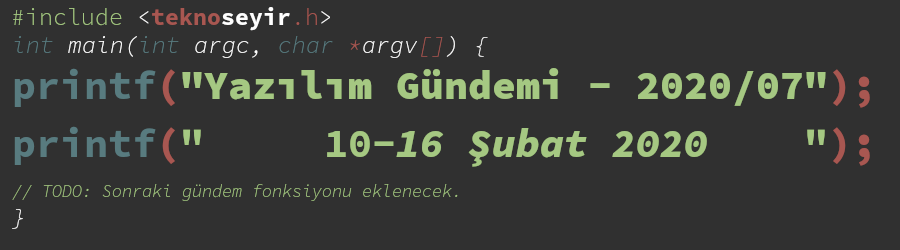
\includegraphics[width=.9\linewidth]{gorseller/yazilim-gundemi-banner.png}
\end{center}

\begin{center}
\href{../06/yazilim-gundemi-2020-06.pdf}{< Önceki Gündem} | \textbf{10-16 Şubat 2020} | \href{../08/yazilim-gundemi-2020-08.pdf}{Sonraki Gündem >}

\href{https://teknoseyir.com/blog/yazilim-gundemi-2020-07}{TeknoSeyir'de Oku}
\end{center}

\section{GitHub komut satırı aracının \href{https://github.blog/2020-02-12-supercharge-your-command-line-experience-github-cli-is-now-in-beta/}{beta programını tanıttı}}
\label{sec:orge328045}
Komut satırı araçları biz geliştiriciler için olmazsa olmazlardan birisi.
Elbette aramızda pek komut satırı kullanmaktan hoşlanmayanlar da olabilir
fakat mutlaka en az 1 ya da 2 tane komut satırı aracı kullanmak durumundadır.
GitHub da kendi hizmetleri için bir komut satırı aracı çıkardı. Henüz beta
programında olan bu komut satırı aracı ile şunları yapabilmekteyiz:

\begin{itemize}
\item Issue'leri listeleme ve filtreleme
\item Issue sayfasını tarayıcı ile açtırma
\item Pull Request oluşturma
\item Pull Request durumunu yazdırma
\item Pull Request'i bilgisayara checkout yapma
\end{itemize}

Şu an beta programında olduğu için çok stabil çalışmasını beklemek yersiz
fakat ben yine de yazıya birkaç görüntü ekleyebilmek için denedim.

\href{https://cli.github.com/}{Bu sayfadan} işletim sisteminize göre olan kurulum dosyasını indirip,
kuruyorsunuz. Ben Linux için olanı kurdum (\texttt{sudo dpkg -{}-install
	gh-0.5.5-linux-amd64.deb}). Sonrasında bilgisayarınızdaki bir git dizininin
içine giriyorsunuz (elbette remote'lar arasında github olmak zorunda) ve \texttt{gh
	issue list} komutunu çalıştırıyorsunuz. Bu komutu ilk kez çalıştırdığınızda
size "tarayıcınızda github'ı açıp izin vermek için enter tuşuna basın" diyor.
Enter'e bastığınızda ise şöyle bir sayfa açılıyor:

\begin{figure}[htbp]
\centering
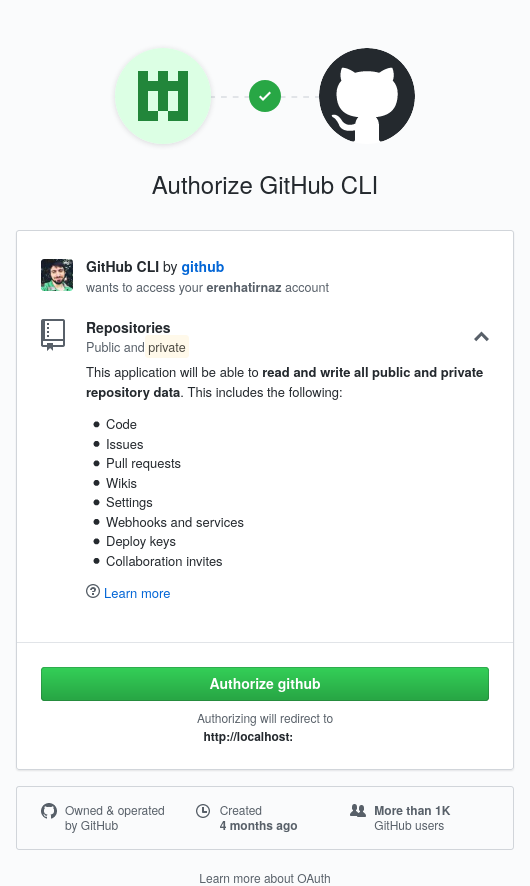
\includegraphics[height=8cm]{gorseller/github-cli-izin.png}
\caption{Görüldüğü gibi bayağı bir izin istiyor ama uygulama zaten GitHub'ın kendine ait olduğu için sıkıntı yok}
\end{figure}
\newpage

GitHub CLI uygulamasına hesabınızın tüm izinlerini verdikten sonra işlem
başarılı olmuşsa sizden bir kere daha Enter tuşuna basmanızı isteyecek ve
bastığınız ise ilgili github deponuzdaki bütün issue girişlerinin listesini
verecek.

\begin{figure}[htbp]
\centering
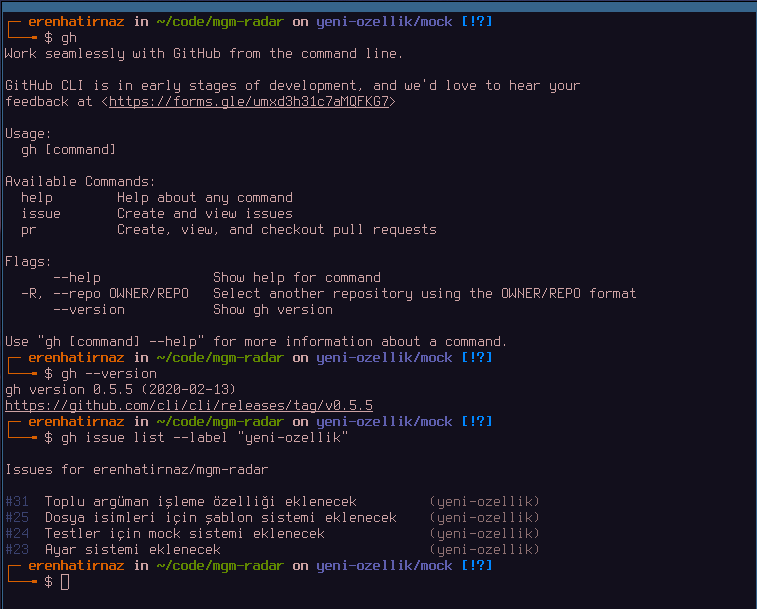
\includegraphics[height=7.5cm]{gorseller/github-cli-demo.png}
\caption{Ben kendi depomda denedim.}
\end{figure}
\newpage

Komut satırı aracında bulduğunuz hataları bildirmek ya da özellik talebinde
bulunmak için bu \href{https://github.com/cli/cli}{github deposunu} ziyaret edebilir ya da \href{https://forms.gle/umxd3h31c7aMQFKG7}{bu formu}
doldurabilirsiniz.

Ayrıca bu hafta içerisinde GitHub, \href{https://github.blog/2020-02-13-github-enterprise-is-now-free-through-microsoft-for-startups/}{Microsoft for Startups hizmeti ile birlikte
GitHub Enterprise çözümünün ücretsiz sunulacağı}nı da duyurdu.
\section{Tembel resim yükleme (lazy-loading) özelliği \href{https://github.com/whatwg/html/pull/3752\#issuecomment-585202516}{HTML standardı oldu}}
\label{sec:org56093a9}
\begin{center}
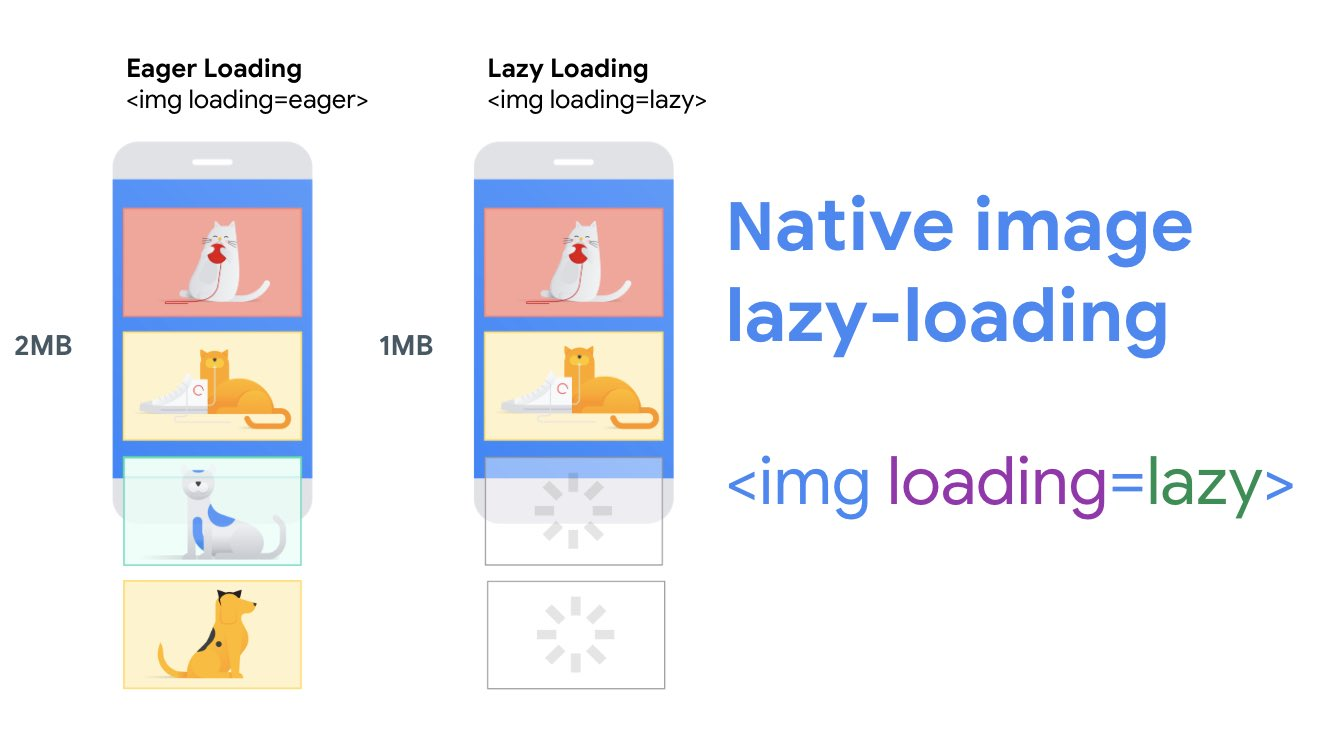
\includegraphics[height=5cm]{gorseller/lazy-loading.png}
\end{center}

Türkçeye çevirince biraz komik bir ifade oldu ama İngilizcesinden anlaşıldığı
üzere bu özellik sayesinde artık bir web sayfasını açtığınızda tüm resimler
aynı anda yüklenmeyecek resimin konumuna göre sayfa scroll edildikte
yüklenecekler. Böylece gereksiz trafik oluşturmaktan kurtulacağız. Hali
hazırda bu özelliği zaten birçok web sitesinde görmüşsünüzdür fakat artık
bunun için ekstra bir kütüphane ya da araça gerek kalmayacak, doğrudan
tarayıcı tarafından desteklenecek.

Bu özelliği kullanmak için HTML kodlarımızı bu şekilde düzenlememiz yeterli
olacak:
\begin{minted}[breaklines=true,breakanywhere=true,frame=lines, linenos, label=HTML]{html}
<img loading=lazy src="img/teknoseyir.png">
\end{minted}

Özellik hakkında detaylı bilgi almak için \href{https://web.dev/native-lazy-loading/}{şu blog yazısı}nı okuyabilirsiniz.

Özelliğin HTML standardı olduğunu duyuran Google Chrome çalışanının \href{https://twitter.com/addyosmani/status/1227619409625174016}{tweet'ine
ise şuradan ulaşabilirsiniz}.
\section{Windows Terminal Preview v0.9 \href{https://devblogs.microsoft.com/commandline/windows-terminal-preview-v0-9-release/}{yayınlandı}}
\label{sec:orgf258fc4}
Microsoft'un yaklaşık bir yıldır geliştirmeye devam ettiği yeni Windows
Terminal uygulamasının v0.9 Önizleme sürümü bu hafta içerisinde duyuruldu.

Bu sürüm ile birlikte artık komut satırından da yeni bir Windows Terminal
penceresi oluşturabiliyoruz. Üstelik oluşturulan bu yeni terminal penceresini
yeni sekme, bölümlenmiş ekran gibi özelliklerle birlikte de oluşturabiliyoruz.
Yani tek bir komut ile terminal sekmesini istediğiniz parçalara bölüp o
parçalarda istediğiniz uygulamaları çalıştırabilirsiniz.

Örneğin önce sekmeyi ortadan ikiye dikey bölüp, sonra da sağ tarafı ortadan
ikiye yatay bölmek için şöyle bir komut çalıştırabilirsiniz:
\begin{minted}[breaklines=true,breakanywhere=true,frame=lines, linenos]{shell}
wt -d C:\Users\cinnamon\GitHub\WindowsTerminal ; split-pane -p "Command Prompt" ; split-pane -p "Ubuntu" -d \\wsl$\Ubuntu\home\cinnak -H
\end{minted}

Bu komutun çıktısı ise şu şekilde:
\url{gorseller/windows-terminal-v09.gif}

Ayrıca bir terminal penceresini kapatmak istediğinizde her zaman "tüm sekmeler
kapatılsın mı" sorusunu sormasın istiyorsanız bunun için de bir ayar eklendi.
Bunu etkinleştirmek için Windows Terminal ayarlarına şu satırı eklemeniz
yeterli:
\begin{minted}[breaklines=true,breakanywhere=true,frame=lines, linenos, label=JSON, labelposition=topline]{json}
"confirmCloseAllTabs": "true"
\end{minted}
Böylece terminal penceresini kapatmak istediğinizde tüm sekmeler de hemen
kapatılacak.
\section{Qt 5.15 Alpha \href{https://www.qt.io/blog/qt-5.15-alpha-released}{sürümü yayınlandı}}
\label{sec:orgc0577e1}
C++ ile platformlar-arası uygulama geliştirmeye yarayan framework Qt'nin 5.15
Alpha sürümü bu hafta içerisinde yayınlandı. Henüz Alpha seviyesinde olması
nedeniyle çalışan uygulamalarınızı bu sürüme yükseltmeniz tavsiye edilmiyor
ama farklı projelerde kullanıp, bulduğunuz hataları Qt takımına
raporlayabilirsiniz. Bu sürüm ile birlikte gelen yeni özellikler için \href{https://wiki.qt.io/New\_Features\_in\_Qt\_5.15}{bu wiki
sayfasını} ziyaret edebilirsiniz.

Ayrıca Qt 5.14.0 sürümüyle birlikte artık "yeniden konumlandırılabilir" oldu.
Ben de ilgili blog yazısının başlığını okuyunca anlamamıştım ama yazıyı
okuyunca fark ettim ki aslında kast edilen: Qt'nin kurulduğunu dizini
değiştebilirsiniz. Böyle bir ihtiyacınız varsa \href{https://www.qt.io/blog/qt-is-relocatable}{bu blog yazısı}nı
okuyabilirsiniz.

Son olarak da KDAB geçtiğimiz sene düzenlediği Qt World Summit 2019
etkinliğinin tüm videolarını bu hafta içerisinde paylaşmış. İlgili duyuru
yazısı için \href{https://www.kdab.com/qt-world-summit-2019-talk-videos-are-online/}{buraya} tıklayabilirsiniz.
\section{Yaklaşan Etkinlikler}
\label{sec:org9165b97}
\begin{longtable}{|p{8cm}|l|l|}
\hline
Etkinlik İsmi & Yeri & Tarihi\\
\hline
\endfirsthead
\multicolumn{3}{l}{Önceki sayfadan devam ediyor} \\
\hline

Etkinlik İsmi & Yeri & Tarihi \\

\hline
\endhead
\hline\multicolumn{3}{r}{Devamı sonraki sayfada} \\
\endfoot
\endlastfoot
\hline
\href{https://www.meetup.com/Microsoft-Giri\%25C5\%259Fimcilik-Bulu\%25C5\%259Fmalar\%25C4\%25B1/events/268435933/}{Azure Serverless Architecture} & İstanbul & 17 Şubat 19:00\\
\href{https://www.meetup.com/istanbul-yapay-zeka-toplulugu/events/268718822/}{Fuat Beşer ile "Yapay Zekâda Öncü Olmak"} & İstanbul & 18 Şubat 14:00\\
\href{https://www.meetup.com/istanbul-yapay-zeka-toplulugu/events/268768436/}{Let The Machine Learn} & İstanbul & 18 Şubat 17:00\\
\href{https://www.meetup.com/GDG-Cloud-Izmir/events/268271805/}{Firebase Study Jam} & İzmir & 18 Şubat 18:00\\
\href{https://www.meetup.com/Teknopark-\%25C4\%25B0stanbul-Yaz\%25C4\%25B1l\%25C4\%25B1mc\%25C4\%25B1-Bulu\%25C5\%259Fmalar\%25C4\%25B1/events/268624461/}{Selenium ve Robot Framework ile UI Test Otomasyonuna Giriş} & İstanbul & 19 Şubat 12:30\\
\href{https://www.meetup.com/IBMDeveloperTR/events/268626077/}{Yapay Zeka ile Dokümanlarınızı Analiz Edin!} & İstanbul & 20 Şubat 19:00\\
\href{https://kommunity.com/devnot-yazilimci-bulusmalari/events/coklu-cluster-ortaminda-cicd-pipeline-ile-uygulama-yonetimi}{Çoklu Cluster Ortamında CI/CD Pipeline ile Uygulama Yönetimi} & İstanbul & 21 Şubat 18:30\\
\href{https://www.eventbrite.com/e/ieee-turkey-2nd-comsoc-conference-tickets-94153113497}{IEEE Turkey 2nd ComSoc Conference} & İstanbul & 22 Şubat 09:30\\
\href{https://www.eventbrite.com/e/deep-learning-fundamentals-workshop-tickets-94146818669}{Deep Learning Fundamentals workshop} & Ankara & 23 Şubat 10:00\\
\href{https://www.meetup.com/rladies-istanbul/events/268481383/}{Shiny Paketi ile Dashboard Hazirlama} & İstanbul & 23 Şubat 12:30\\
\href{https://www.meetup.com/Microsoft-Giri\%25C5\%259Fimcilik-Bulu\%25C5\%259Fmalar\%25C4\%25B1/events/268504659/}{Microservice with Azure Kubernetes Service and Azure Devops} & İzmir & 25 Şubat 13:00\\
\href{https://www.eventbrite.co.uk/e/rdtech-registration-94626158387}{RDTech Solid \& Unit Testing} & İstanbul & 26 Şubat 18:00\\
\href{https://kommunity.com/jamstack/events/jamstack-istanbul}{JAMstack Istanbul} & İstanbul & 26 Şubat 19:00\\
\href{https://www.meetup.com/Sahibinden-D2D-Events/events/268634768/}{Kotlin ve Java'nın Yeni Versiyonları} & İstanbul & 26 Şubat 19:00\\
\href{https://www.eventbrite.com/e/testdefence-yuksek-kaliteli-guvenilir-savunma-sistemleri-ve-yazlmlar-nasl-gelistirilir-tickets-88086646531}{TestDefence: Yüksek Kaliteli, Güvenilir Savunma Sistemleri ve Yazılımları Nasıl Geliştirilir?} & Ankara & 27 Şubat 13:00\\
\href{https://www.meetup.com/Microsoft-Giri\%25C5\%259Fimcilik-Bulu\%25C5\%259Fmalar\%25C4\%25B1/events/268504693/}{Microservice with Azure Kubernetes Service and Azure Devops} & Ankara & 27 Şubat 13:00\\
\href{https://www.eventbrite.com/e/codeyapkredi-vol-4-ses-teknolojilerinin-yarattg-degisim-ve-podcast-tickets-94125416655}{Code.YapıKredi Vol 4: Ses Teknolojilerinin Yarattığı Değişim ve Podcast} & İstanbul & 27 Şubat 19:00\\
\href{https://www.eventbrite.com/e/siber-guvenlikte-yapay-zeka-tickets-92908165825}{Siber Güvenlikte Yapay Zeka} & Ankara & 27 Şubat 19:00\\
\href{https://www.meetup.com/Hepsitech-Meetup/events/268530407/}{Hepsiburada Micro Frontends Dönüşümü} & İstanbul & 27 Şubat 19:00\\
\href{https://www.meetup.com/Javascript-Ankara/events/268677048/}{JS Ankara Şubat 2020 Etkinliği} & Ankara & 27 Şubat 19:00\\
\href{https://kommunity.com/cloud-and-serverless-turkey/events/the-future-of-real-time-offline-data-istanbul}{The Future of Real-time - Offline - Data} & İstanbul & 28 Şubat 18:30\\
\href{https://www.eventbrite.com/e/geekday-2020-tickets-93463962227}{GeekDay 2020} & Kocaeli & 29 Şubat 09:00\\
\href{https://www.meetup.com/GDGKocaeli/events/268678688/}{Tensor Flow Study Jam} & Kocaeli & 29 Şubat 13:00\\
\href{https://kommunity.com/freecodecamp-istanbul/events/freecodecamp-istanbul-tanitim-etkinligi}{freeCodeCamp İstanbul Tanıtım Etkinliği} & İstanbul & 29 Şubat 14:00\\
\href{https://kommunity.com/bilge-adam-teknoloji/events/tensorflow}{TensorFlow Fest (TensorFlow Turkey)} & Ankara & 1 Mart 10:00\\
\href{https://www.meetup.com/GDG-Manisa/events/268736708/}{Firebase Study Jam} & Manisa & 3 Mart 12:00\\
\href{https://kommunity.com/devops-turkiye/events/prometheus-ve-grafana-ile-metrik-olusturma-ve-goruntuleme}{Prometheus ve Grafana ile Metrik Oluşturma ve Görüntüleme} & İstanbul & 4 Mart 18:30\\
\href{https://www.meetup.com/Microsoft-Giri\%25C5\%259Fimcilik-Bulu\%25C5\%259Fmalar\%25C4\%25B1/events/268504717/}{Microservice with Azure Kubernetes Service and Azure Devops} & İstanbul & 5 Mart 13:00\\
\href{https://www.meetup.com/QWomen-\%25C4\%25B0stanbul/events/268233749/}{Kuantum Programlamaya Giriş Atölyesi} & İstanbul & 7 Mart 09:00\\
\href{https://www.meetup.com/gdgtekirdag/events/268421016/}{WTM Tekirdağ IWD 2020} & Tekirdağ & 7 Mart 10:00\\
\href{https://www.meetup.com/GDG-Cloud-Istanbul/events/268749560/}{Google Cloud Run Workshop} & İstanbul & 7 Mart 14:00\\
\href{https://www.meetup.com/GDG-Cloud-Izmir/events/268749612/}{GCP Projects, Service Account And Billing \& Intro to Computing in GCP} & İzmir & 8 Mart 13:00\\
\hline
\end{longtable}
\section{Diğer Haberler}
\label{sec:org2597048}
\begin{itemize}
\item DeepMind, yapay zekada uzun dönem hafıza araştırmaları için \href{https://deepmind.com/blog/article/A\_new\_model\_and\_dataset\_for\_long-range\_memory}{yeni bir model
ve veri seti yayınladı}.
\item GitHub, resmi olarak \href{https://github.blog/2020-02-12-announcing-github-india/}{Hindistan'a girdi}.
\item Microsoft Azure takımı, büyük git depoları için \href{https://devblogs.microsoft.com/devops/introducing-scalar/}{optimizasyon çözümünü
tanıttı}: \href{https://github.com/microsoft/scalar/}{Scalar}.
\item .NET Core takımı native WPF komponentlerini \href{https://github.com/dotnet/wpf/issues/2554}{açık kaynak yaptı}.
\item Netflix, \href{https://aomediacodec.github.io/av1-avif/}{AVIF resim formatı} için hazırladığı sıkıştırma karşılaştırma
aracını \href{https://netflixtechblog.com/avif-for-next-generation-image-coding-b1d75675fe4}{açık kaynak olarak yayınladı}: \href{https://github.com/Netflix/image\_compression\_comparison}{netflix/image-compression-comparion}
\item Facebook ve Social Science One, milyonlarda facebook URL'sinden oluşan veri
setini \href{https://socialscience.one/blog/unprecedented-facebook-urls-dataset-now-available-research-through-social-science-one}{akademik çalışmalar için yayınladı}.
\item Google, Samsung'u Android çekirdeğinde gereksiz değişiklikler yaparak
\href{https://9to5google.com/2020/02/14/google-samsung-android-kernel-changes-security/}{zaafiyetlere yol açmakla itham ediyor}. Google Project Zero takımının \href{https://googleprojectzero.blogspot.com/2020/02/mitigations-are-attack-surface-too.html}{detaylı
blog yazısı}
\item Google Yapay Zeka takımı, video boyutlarını otomatik olarak akıllı şekilde
kırpabilen aracını \href{https://ai.googleblog.com/2020/02/autoflip-open-source-framework-for.html}{açık kaynak olarak yayınlandı}: \href{https://github.com/google/mediapipe/blob/master/mediapipe/docs/autoflip.md}{AutoFlip}.
\item Google kendi bellek ayırma kütüphanesi TCMalloc'u \href{https://abseil.io/blog/20200212-tcmalloc}{açık kaynak olarak
yayınladı}. \href{https://github.com/google/tcmalloc}{GitHub Deposu}
\item ING Bank, web komponentleri kütüphanesini \href{https://medium.com/ing-blog/ing-open-sources-lion-a-library-for-performant-accessible-flexible-web-components-22ad165b1d3d}{açık kaynak hale getirdi}: \href{https://github.com/ing-bank/lion}{Lion}.
\item Yeni bir sıralama algoritması tanıtıldı: \href{https://github.com/scandum/quadsort}{quadsort}.
\item Go programlama dilinin 1.13.8 ve 1.12.17 \href{https://golang.org/doc/devel/release.html\#go1.13.minor}{sürümleri yayınlandı}.
\item Crystal programlama dilinin 0.33.0 \href{https://crystal-lang.org/2020/02/14/crystal-0.33.0-released.html}{sürümü yayınlandı}.
\item Racket programlama dilinin 7.6 \href{https://download.racket-lang.org/v7.6.html}{sürümü yayınlandı}.
\item Delphi 25 \href{https://community.idera.com/developer-tools/b/blog/posts/25-years-of-excellence}{yaşına girdi}.
\item Spring framework web \href{https://spring.io/blog/2020/02/14/announcing-the-new-spring-website}{sitesini güncelledi}.
\item Redux Toolkit v1.3.0-Alpha.5 \href{https://github.com/reduxjs/redux-toolkit/releases/tag/v1.3.0-alpha.5}{sürümü yayınlandı}.
\item Uzak Git deposu sunucu Gitea 1.11.0 \href{https://blog.gitea.io/2020/02/gitea-1.11.0-is-released/}{sürümünü yayınladı}.
\item OpenSSH 8.2 \href{https://lists.mindrot.org/pipermail/openssh-unix-announce/2020-February/000138.html}{sürümü yayınlandı}.
\item Apache Flink 1.10 \href{https://flink.apache.org/news/2020/02/11/release-1.10.0.html}{sürümü yayınlandı}.
\item PostgreSQL 12.2, 11.7, 10.12, 9.6.16, 9.5.21 ve 9.4.29 \href{https://www.postgresql.org/about/news/2011/}{sürümleri yayınlandı}.
\item \href{https://openchakra.app/}{OpenChakra} aracının ilk stabil versiyonu 1.0.0 \href{https://github.com/premieroctet/openchakra/releases/tag/v1.0.0}{çıktı}.
\item GDBFrontend v0.0.16-alpha \href{https://github.com/rohanrhu/gdb-frontend/releases/tag/v0.0.16-alpha}{sürümü çıktı}.
\item KDE Frameworks 5.67.0 \href{https://kde.org/announcements/kde-frameworks-5.67.0.php}{sürümü çıktı}.
\end{itemize}
\section{Lisans}
\label{sec:org752b4b5}
\begin{center}
\begin{center}

\includegraphics[height=1.5cm]{../../../img/CC_BY-NC-SA_4.0.png}
\end{center}

\href{yazilim-gundemi-2020-07.pdf}{Yazılım Gündemi - 2020/07} yazısı \href{https://erenhatirnaz.github.io}{Eren Hatırnaz} tarafından \href{http://creativecommons.org/licenses/by-nc-sa/4.0/}{Creative Commons
Atıf-GayriTicari-AynıLisanslaPaylaş 4.0 Uluslararası Lisansı} (CC BY-NC-SA 4.0)
ile lisanslanmıştır.
\end{center}
\end{document}
